\subsection{Muon systems}

%Finally, there is the muon system.
%Each station uses Multi-Wire Projection Chambers exclusively, except for the centre of M1, where
%the expected flux would age this technology too quickly; in this area Gas Electron Multiplier
%detectors are used.
%Like the calorimeters, the muon stations have increased cell density near the beam; however in
%contrast, the cell density is greater in the bending plane than the non-bending plane in order to
%increase momentum resolution.
%Only muon stations M2-5 are used for particle identification; theses are interleaved with plates of
%$80\cm$ thick lead plates, so only very energetic muons reach M5.
%For this reason M4 and M5 are used to identify these penetrating muons, while M2 and M3 have
%increased single hit resolution for momentum measurements.
%In many \lhcb analyses a muon is identified based on hits within the muon system, the criteria is
%known as {\tt isMuon}.
%It is defined as follows: particles with momenta $3<p<6\gev$ must be associated with hits in M2 and M3; if
%$6<p<10\gev$ there must be hits in M2, M3 and either M4 or M5; else if $p>10\gev$ there must be
%associated hits in all M2--5.


Muons are the only charged particles enetracting enough to poass through the calorimeter system.
Muons contribute to the final state of many $b$-hadron decays, including \lhcb{s} flagship
measurements of  the branching fraction \decay{\Bs}{\mumu} and the angular analysis of
\decay{\Bd}{\Kstarz\mumu}.
The muon system is designed to give precise measurements of muon trajectories and triggering of
decays with muons in the final state.

The muon system consists of five muon stations, M1--5.
The first station, M1, is located directly upstream of the calorimeters; the other stations are all
downstream of the calorimetery system and are interleaved with $80\cm$ thick iron absorbers.
Layout of the \lhcb muon system is shown in \Fig{fig:lhcb:muonside}.

\begin{figure}
  \begin{center}
    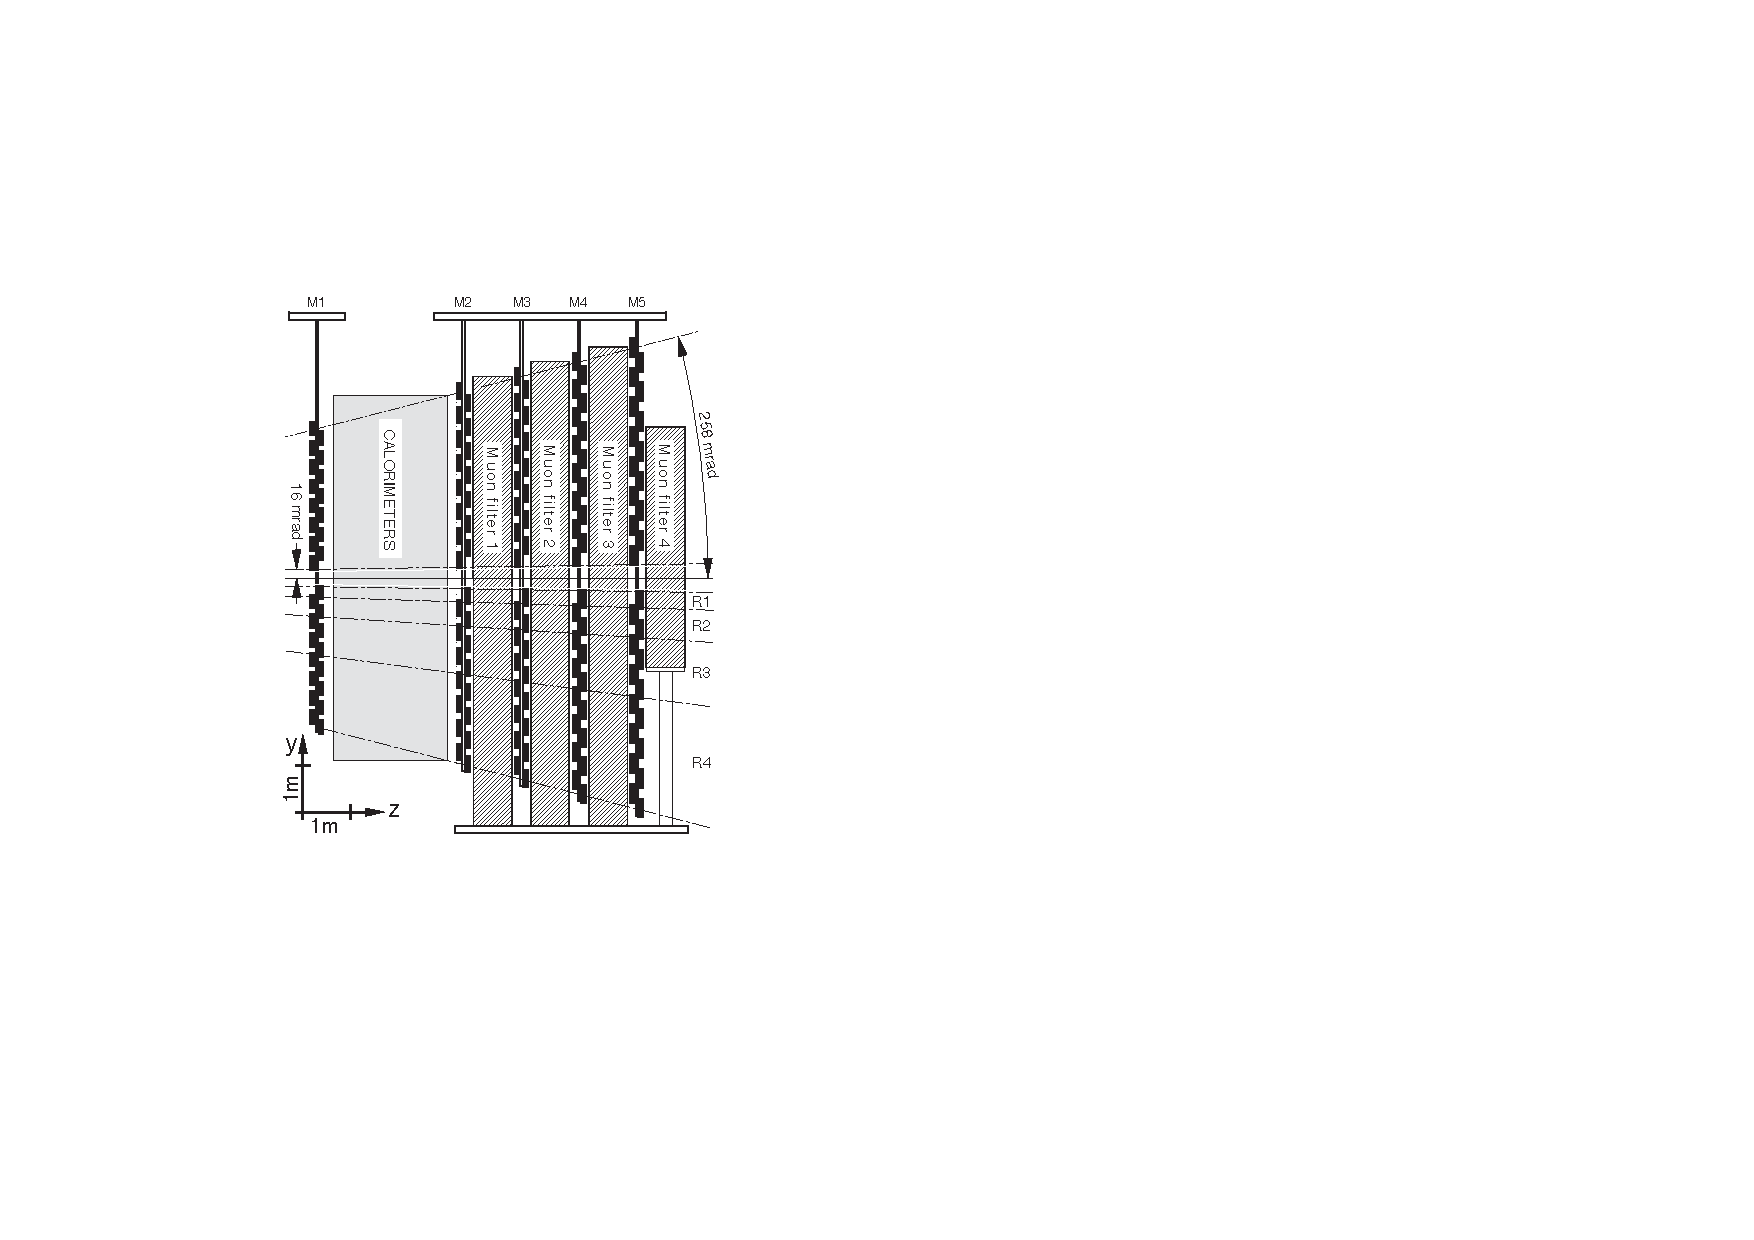
\includegraphics[width=0.48\textwidth]{muonside}
    \caption[Side view of the LHCb muon system]
    {\small
      Side-on view of the LHCb muon system.
      The M1 station is located upstream of the calorimeters, and M2--5 are all downstream.
      Relative scales are the same, but absolute dimensions scale with distance from the $pp$
      interaction point, such that the angular coverage is identical for each station.
      Between stations M2--5 are $80\cm$ thick iron filters.
      Regions R1--4 indicate where the resolution is the same, this is shown clearly in
      Fig.~\protect\ref{fig:lhcb:muonpad}.
    }
    \label{fig:lhcb:muonside}
  \end{center}
\end{figure}

Each station uses Multi-Wire Projection Chambers, except for the centre of M1, where
the expected muon flux would age this technology too quickly; in this area Gas Electron Multiplier
detectors are used.
Detector resolution is defined by rectangular logical pads, which have varying spacial resolutions,
becoming courser as the distance from the beam axis increases.
These regions are discretized, and labelled R1--4 as shown in Figure~\ref{fig:lhcb:muonpad},
where the segmentation ratios for $\mathrm{R}1:\mathrm{R}2:\mathrm{R}3:\mathrm{R}4$ are $1:2:4:8$,
such that the flux in each region is approximately equal.
The number of detection cells in the bending plane is greater than in the non-bending plane, in
order to increase the momentum resolution.
The inclusion of the M1 station is primarily to provide improved momentum resolution in the
trigger, giving a momentum resolution of approximately $20\pc$.
In total, the absorber material is 20 interaction lengths, such that only highly penetrating muons
reach M4--5, in order to pass through all the muon stations a muon must have a \pt of at least
$6\gev$.
Therefore, stations M1--3 have excellent spacial resolution, whereas the stations M4--5 are
primarily used for identifying highly penetrating muons.

\begin{figure}
  \begin{center}
    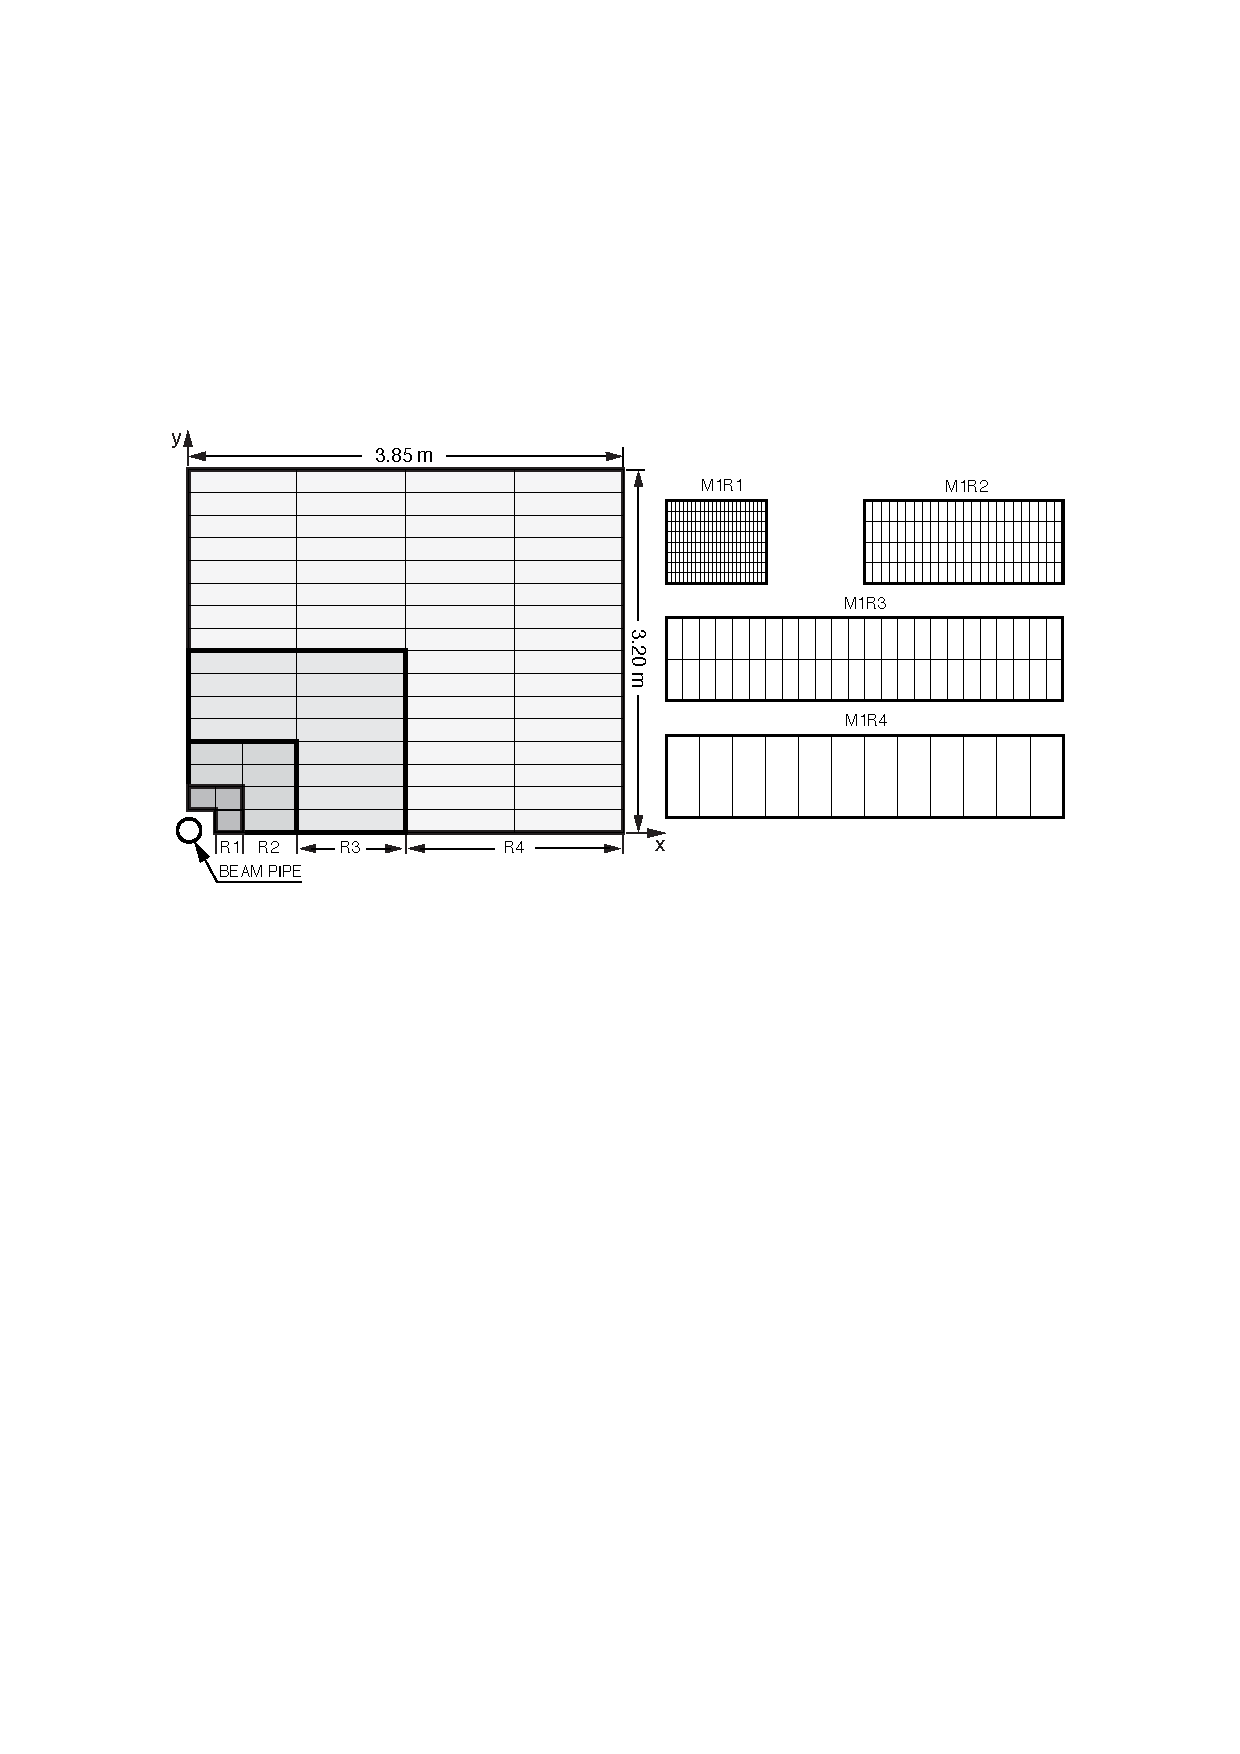
\includegraphics[width=0.98\textwidth]{muon1}
    \caption[Front view of the LHCb muon system]
    {\small
      Front-on view of a single quadrant of a muon station.
      The left-hand pane shows the chambers distributed throughout regions R1--4.
      Each chamber comprises a logical pad structure as shown for M1 in the right-hand diagram.
      The resolution for the stations in M2--3(M4--5) are double(half) that of M1.
    }
    \label{fig:lhcb:muonpad}
  \end{center}
\end{figure}

The muon system provides important \pid information.
In many \lhcb analyses a muon is identified based on hits within the muon system, the criteria is
known as {\tt isMuon}.
The criteria is dependent upon the muon momentum, and defined exactly in \Tab{tab:lhcb:ismuon}.

\begin{table}
  \caption{\small
    The {\tt isMuon} flag is an important variable used to identify muons.
    The criteria depends on the particle's measured momentum.
    If the {\tt isMuon} condition returns a true then the particle is identified to be a muon.
  }
  \label{tab:lhcb:ismuon}
  \begin{center}
    \begin{tabular}{cl}
      \toprule
      $p(\mu)$ range (GeV)& \cellc{{\tt isMuon} condition} \\
      \midrule
      \makebox[\widthof{$6<p(\mu)<10$}][r]{$3<p(\mu)<\pz6$}
      & M2 and M3 \\
      \makebox[\widthof{$6<p(\mu)<10$}][r]{$6<p(\mu)<10$}
      & M2 and M3 and (M4 or M5) \\
      \makebox[\widthof{$6<p(\mu)<10$}][r]{$p(\mu)>10$}
      & M2 and M3 and M4 and M5 \\
      \bottomrule
    \end{tabular}
  \end{center}
\end{table}
